% File: CableTension1.tex
% Author: Adam Leeper
%------------------------------------------------------------------------------
\providecommand{\isolatedBuild}[1]{#1}% Fallback definition to build normally.
\isolatedBuild{
  \documentclass[11pt,letterpaper]{book}
  %\documentclass[11pt,letterpaper]{book}

% aleeper: I think these are needed for Paul's macros?
\usepackage{epsfig}
\usepackage{epstopdf}

%\makeatletter
%\typeout{The import path is \import@path}
%\makeatother

\usepackage{import}

\subimport{./}{packagesMitiguy.sty}
\subimport{./}{macrosMitiguy.tex}
\subimport{./}{PageStylesMitiguy.tex}
\subimport{./}{macrosLeeper.tex}
   % Found via TEXINPUTS environment variable.
  \isolatedBuildHeader{Vector Basics: Measures and Components}
                      {Force Measures for Cables on a Concrete Support}
                      %\footnote{Adapted from problem 2.7.13 of Sheri Sheppard's textbook.}}
}
%%%
%%%
%%%
\begin{minipage}[t]{0.6\linewidth}
  \minipageTopAnchor
  (Adapted from problem 2.7.13 of Sheri Sheppard's textbook.)
  %
  \\[0.45pc]
  The figure at right shows two cables tethered to a support at point $O$.
  The tension in the left cable is $\tension{1} = 2$ kip, and the tension in the
  right cable is $\tension{2} = 1$ kip (1 kip \equals[\;] 1000 lb-force).
  %
  \\[0.45pc]
  The support is embedded in concrete, which is very strong in compression but
  relatively weak in tension.
  Engineers are concerned that the support will pull out of the concrete if
  the force pulling perpendicular to the concrete surface
  (along the axis of the support, up-and-right) exceeds 2500 lb-force.
\end{minipage}
\begin{minipage}[t]{0.4\linewidth}
  \minipageTopAnchor
  \centering
  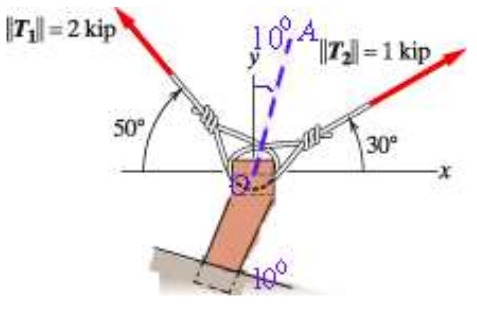
\includegraphics[width=6cm]{sheppard_2-7-13.jpg}
\end{minipage}

\begin{enumerate}
  \item
    Determine the resultant force at $O$ due to the cables. Express your
    answer in terms of \uvecHat{x} and \uvecHat{y} components, and then
    also in components parallel and perpendicular to the concrete surface.
    Note: Use the \textit{definition} of dot-product.
    %
    \\[0.45pc]
    \Solution{}{0.97\linewidth}{
      To aid in bookkeeping and to let us work with a \textit{simple}
      expression, we define unit vectors in the direction of each
      cable: \uvecHat{u} in the direction of cable 1, and \uvecHat{w} in the
      direction of cable 2.
      %
      The resultant force due to the cables is then:
      $$\force{O} \equals[\;]
        \tension{1} \uvecHat{u} \plus[\;] \tension{2} \uvecHat{w}$$
      %
      This is the simplest possible expression of $\force{O}$.
      It is uncommitted to any particular components or measures.
      \\[0.45pc]
      %
      \textbf{Horizontal and Vertical components:}
      \\[0.2pc]
      To express this vector in horizontal and vertical components, we can dot
      with \uvecHat{x} and \uvecHat{y} to get
      the \textit{measures} of the force in each of those directions.
      The angles in each dot-product are obtained by inspection of the figure.
      %
      \\[0.45pc]
      \begin{tabular}{ll@{\equals[\;]}l}
        %\text{dot with \uvecHat{x}:}
        & $\force{O} \DotProduct[\;] \uvecHat{x}
          \equals[\;] (\tension{1} \uvecHat{u} \plus[\;] \tension{2} \uvecHat{w})
          \DotProduct[\;] \uvecHat{x}
          \equals[\;] \tension{1} ~\uvecHat{u} \DotProduct[\;] \uvecHat{x}
            \plus[\;] \tension{2} ~\uvecHat{w} \DotProduct[\;] \uvecHat{x}
          \equals[\;] \tension{1} \cos(\degrees{130})
            \plus[\;] \tension{2} \cos(\degrees{30})$
        & $-0.420 \text{~kip}$
        \\[0.45pc]
        %\text{dot with \uvecHat{y}:}
        & $\force{O} \DotProduct[\;] \uvecHat{y}
          \equals[\;] (\tension{1} \uvecHat{u} \plus[\;] \tension{2} \uvecHat{w})
          \DotProduct[\;] \uvecHat{y}
          \equals[\;] \tension{1} ~\uvecHat{u} \DotProduct[\;] \uvecHat{y}
            \plus[\;] \tension{2} ~\uvecHat{w} \DotProduct[\;] \uvecHat{y}
          \equals[\;] \tension{1} \cos(\degrees{40})
            \plus[\;] \tension{2} \cos(\degrees{60})$
        & $2.03 \text{~kip}$
      \end{tabular}
      %
      \\[0.45pc]
      Hence \force{O} can be written as:
      $$\force{O} \equals[\;] -0.420 \text{~kip~} \uvecHat{x} \plus[\;]
                               2.03  \text{~kip~} \uvecHat{y}$$
      %
      %
      \textbf{Components parallel and perpendicular to concrete surface:}
      \\[0.2pc]
      To aid in bookkeeping, we define a new set of orthogonal unit vectors
      with \uvecx{c} pointed parallel to the surface (down-and-right), and \uvecy{c}
      pointed perpendicular to the surface (up-and-right).
      \\[0.45pc]
      As before, to obtain the \uvecx{c} and \uvecy{c} \textit{measures} of the
      force we simply dot with each of these unit vectors.
      The angles in each dot-product are obtained by inspection of the figure.
      %
      %
      \\[0.45pc]
      \begin{tabular}{ll@{\equals[\;]}l}
        %\text{dot w/ \uvecx{c}:}
        & $\force{O} \DotProduct[\;] \uvecx{c}
          \equals[\;] (\tension{1} \uvecHat{u} \plus[\;] \tension{2} \uvecHat{w})
          \DotProduct[\;] \uvecx{c}
          \equals[\;] \tension{1} ~\uvecHat{u} \DotProduct[\;] \uvecx{c}
            \plus[\;] \tension{2} ~\uvecHat{w} \DotProduct[\;] \uvecx{c}
          \equals[\;] \tension{1} \cos(\degrees{140})
            \plus[\;] \tension{2} \cos(\degrees{40})$
        & $-0.766 \text{~kip}$
        \\[0.45pc]
        %\text{dot w/ \uvecy{c}:}
        & $\force{O} \DotProduct[\;] \uvecy{c}
          \equals[\;] (\tension{1} \uvecHat{u} \plus[\;] \tension{2} \uvecHat{w})
          \DotProduct[\;] \uvecy{c}
          \equals[\;] \tension{1} ~\uvecHat{u} \DotProduct[\;] \uvecy{c}
            \plus[\;] \tension{2} ~\uvecHat{w} \DotProduct[\;] \uvecy{c}
          \equals[\;] \tension{1} \cos(\degrees{50})
            \plus[\;] \tension{2} \cos(\degrees{50})$
        & $1.93 \text{~kip}$
      \end{tabular}
      %
      \\[0.45pc]
      Hence \force{O} can be written as:
      $$\force{O} \equals[\;] -0.766 \text{~kip~} \uvecx{c} \plus[\;]
                               1.93  \text{~kip~} \uvecy{c}$$
      %
    }
    %
  \item Use your results from the previous part to analyze the situation and
    determine if failure will occur.
    %
    \\[0.45pc]
    \Solution{}{0.97\linewidth}{
      The engineers are concerned about the ``force pulling along the axis of
      the support", which in our analysis is the \uvecy{c} \textit{measure} of
      $\force{O}$. We found the \uvecy{c} measure to be 1.93 kip \equals[\;]
      1930 lb, so we know the concrete will not fail.
      %
      \\[0.45pc]
      \textbf{Note:} It is \textbf{\underline{not necessary}} to fully resolve a
      vector into components in order to determine one of them. If all we
      really care about is the \uvecy{c} measure of the force, then we simply dot
      with \uvecy{c}:
      $$\text{``force along axis of support"} \equals[\;]
        \force{O} \DotProduct[\;] \uvecy{c}
          \equals[\;] \tension{1} ~\uvecHat{u} \DotProduct[\;] \uvecy{c}
            \plus[\;] \tension{2} ~\uvecHat{w} \DotProduct[\;] \uvecy{c}
          \equals[\;] \tension{1} \cos(\degrees{50})
            \plus[\;] \tension{2} \cos(\degrees{50})
          \equals[\;] 1.93 \text{~kip}$$
    }
    %
\end{enumerate}
%
\isolatedBuildFooter
